% !TEX encoding = UTF-8
% !TEX TS-program = pdflatex
% !TEX root = ../tesi.tex
% !TEX spellcheck = it-IT

%**************************************************************
\chapter{L'Azienda}
\label{cap:azienda}
%**************************************************************

\intro{Il presente capitolo è dedicato alla presentazione dell'Azienda 
	che mi ha ospitato nella propria sede per uno stage obbligatorio
	per la Laurea triennale. \\
	Ho strutturato la presentazione in tre parti: nella 
	prima parte introduco l'azienda, nella seconda parte descrivo il suo profilo 
	aziendale e nello specifico il settore di mercato in cui essa opera, 
	chi sono i suoi clienti, come è strutturata e
	qual è il suo modello di qualità. Infine, descrivo il suo rapporto con 
	l'innovazione.}


%\noindent Esempio di utilizzo di un termine nel glossario \\
%\gls{api}. \\

%\noindent Esempio di citazione in linea \\
%\cite{site:\gls{agile}-manifesto}. \\

%\noindent Esempio di citazione nel pie' di pagina \\
%citazione\footcite{womak:lean-thinking} \\

%**************************************************************
% Introduzione all'azienda 
\section{IKS}
%\vspace{30pt}
%\begin{figure}[htbp]
%	\begin{center}
%		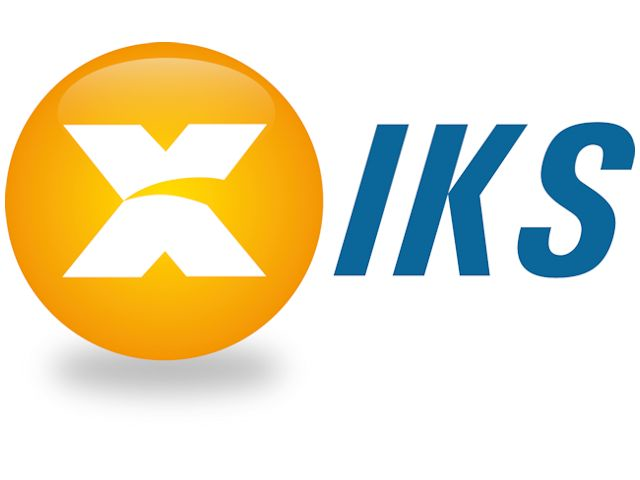
\includegraphics[height=2cm]{iks}
%		\caption{Il logo aziendale}
%	\end{center}
%\end{figure}

%\vspace{30pt}

IKS \emph{(Information Knowledge and Supply)} è un'azienda padovana 
fondata dall'attuale Amministratore Delegato Paolo Pittarello nel 1999. 

Nell'insieme, IKS unisce figure di alto profilo per proporre soluzioni 
innovative alle richieste di mercato dell'\gls{ict} sia italiano che estero. 
Le soluzioni offerte interessano in particolare gli ambiti della sicurezza, 
dell'infrastruttura e della governance \gls{it}.  

L'azienda è in continua ricerca tecnologica. Investendo sulla formazione del 
proprio personale, IKS si impegna di portare solo valore aggiunto al business 
dei propri clienti. Inoltre, l'Azienda crede fortemente nell'innovazione come 
strumento verso un ambiente digitale comune, \gls{agile} e completamente disponibile. 

Il quartier generale aziendale è a Padova. Inoltre, IKS possiede uffici 
anche nelle seguenti città: Roma, Milano e Trento.

A partire dallo scorso anno, 2016, IKS SRL, Kirey SRL, Insirio SPA e 
System Evolution SRL hanno  fondato il Gruppo Kirey. L'obiettivo comune delle 
quattro aziende è unire le competenze complementari e garantire un portfolio 
completo di soluzioni ai clienti attuali e futuri. 

La creazione del Gruppo Kirey è stata guidata dalla Synergo SGR una società di 
\gls{private equity}. E il presidente del nuovo Gruppo commerciale è Vittorio Lusvarghi.   

A seguito della creazione del Gruppo, IKS SRL e le restanti tre realtà aziendali 
hanno conservato la propria struttura di governance e management, garantendo 
la continuità gestionale. 
%**************************************************************

% Parte prima del capitolo
\section{Profilo dell'azienda}
\subsection{Servizi e prodotti offerti}
Nel corso degli anni IKS si è fatta notare per gli enormi contributi innovativi 
nell'ambito della sicurezza informatica. Tuttavia, essa non è limitata a 
questo ambito. Infatti, gli altri ambiti di applicazione sono: infrastruttura e governance IT. 

Di seguito vengono presentati quali sono i servizi offerti da IKS per ciascun ambito:

\begin{itemize}
	\item \textbf{IT Security}\\
	 \begin{itemize}
	 	\item \textbf{Risk analysis e vulnerability assessment}\\ 
	 	E' importante garantire la sicurezza dell'infrastruttura informatica nel suo complesso. 
	 	A questo scopo IKS offre un servizio orientato alla ricerca di eventuali vulnerabilità e 
	 	analisi dei rischi a esse collegate;
	 
	 	\begin{figure}[htbp]
	 		\begin{center}
	 			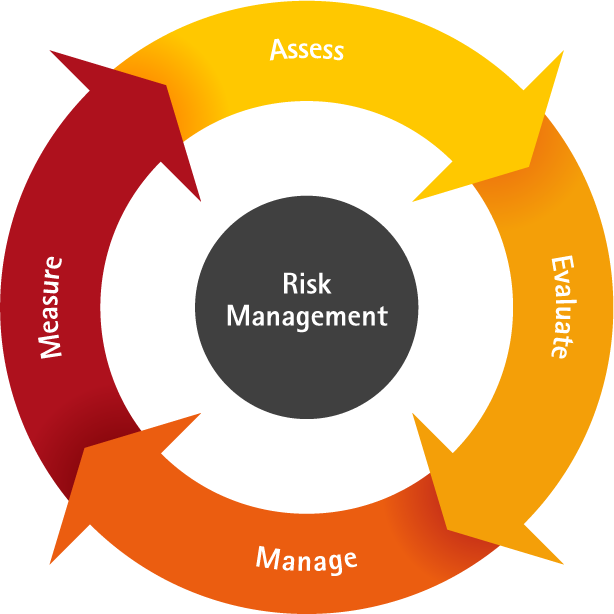
\includegraphics[height=4cm]{risk-management}
	 			\caption{Visione a processo della gestione del rischio. Immagine tratta da: http://bit.ly/2rh3V0A.}
	 		\end{center}
	 	\end{figure}
	 		 	
		\item \textbf{Audit management}\\
		Le aziende di continuo sono sottoposte a controlli di vario genere per accertare che le 
		operazioni aziendali sono a norma con certificazioni, leggi, bilanci ed ecc. A questo 
		scopo IKS offre un servizio di supporto per le aziende con il fine di agevolare le 
		attività di auditing e eventualmente per migliorare i processi interni aziendali;
		\begin{figure}[htbp]
			\begin{center}
				\hspace{3em}
				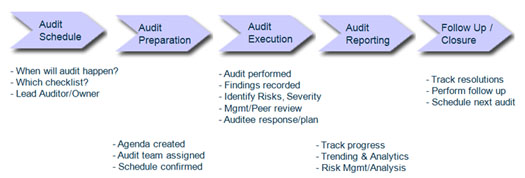
\includegraphics[height=3.5cm]{audit-management}
				\caption{Flusso di lavoro durante lo svolgimento di un audit. Immagine tratta da: http://bit.ly/2rdFhfv.}
			\end{center}
		\end{figure}
	
		\newpage
	 	\item \textbf{Difesa perimetrale}\\ 
	 	Sempre in ambito della sicurezza è importante prendere le giuste misure per garantire 
	 	a priori uno specifico livello di sicurezza e limitare a zero le intrusioni dall'esterno 
	 	di un'infrastruttura IT aziendale. A questo scopo IKS offre un'insieme di soluzioni 
	 	orientare al monitoraggio degli accessi a sistemi aziendali, dei permessi sulle operazioni 
	 	che un utente può fare e/o vedere, e molto altro;
	 	\begin{figure}[htbp]
	 		\begin{center}
	 			
\includegraphics[height=4cm]{firewall}
	 			\caption{Visione grafica del concetto di difesa perimetrale. Immagine tratta da: http://bit.ly/2s834O2.}
	 		\end{center}
	 	\end{figure}
	 	
	 \end{itemize}	
	\item \textbf{IT Infrastructure}\\
	 \begin{itemize}
	 	\item \textbf{Business continuity}\\
	 	In ambito bancario, le infrastrutture informatiche sono molto complesse. E la loro manutenzione 
	 	non è semplice. Ancora più difficile è garantire che questi sistemi siano operativi al 100\%. 
	 	Una simile percentuale nella pratica è impossibile. IKS con il proprio gruppo di esperti 
	 	sono alla continua ricerca di soluzioni per incrementare la percentuale di continuità operativa 
	 	di questi sistemi. Infatti, le soluzioni offerte dall'azienda sono orientate nel concreto all'infrastruttura 
	 	del cliente richiedente supporto;
	 	\begin{figure}[htbp]
	 		\begin{center}
	 			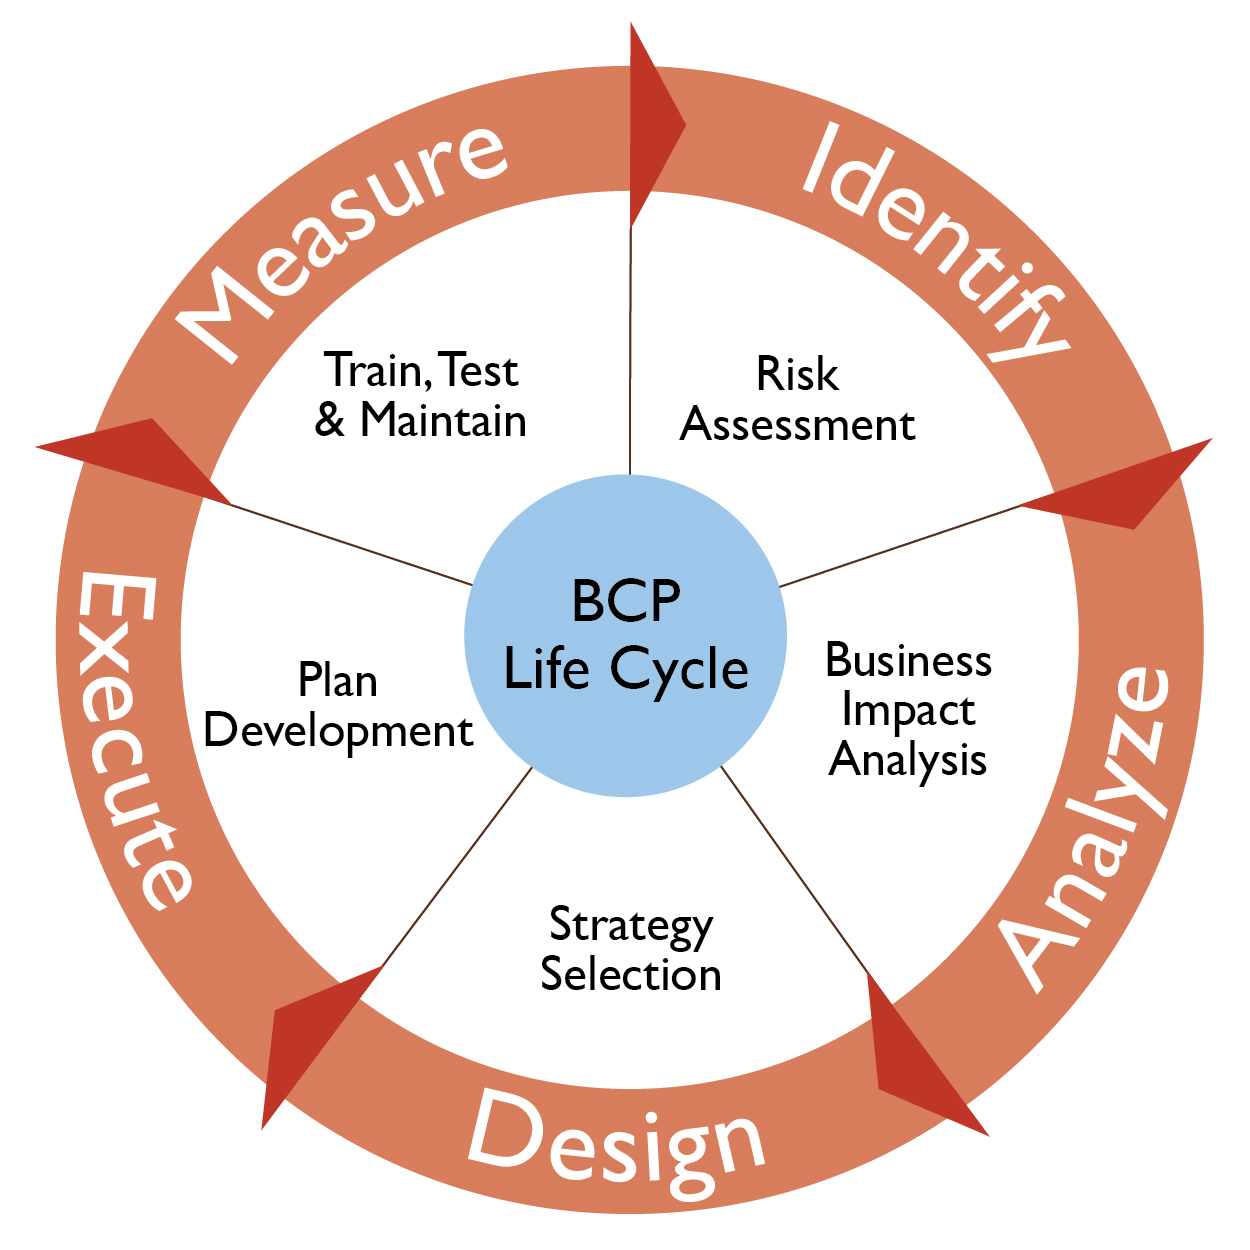
\includegraphics[height=5cm]{business-continuity}
	 			\caption{Visione del ciclo di vita del processo business continuity. Immagine tratta da: http://bit.ly/2qvCmgP.}
	 		\end{center}
	 	\end{figure}
	 \newpage
	 	
	 	\item \textbf{Virtualization technology}\\
	 	Ogni prodotto software per portare valore aggiunto a un'azienda deve essere eseguito. Mappare in 
	 	esecuzione un prodotto software per server fisico richiede la disponibilità di un cospicuo numero 
	 	di questi server. A questo scopo la tecnologia di virtualizzazione permette la creazione di server logici 
	 	che eseguono programmi e a loro volta vanno in esecuzione su server fisici. I benefici di una simile 
	 	infrastruttura è l'ottimizzazione delle risorse di calcolo, agilità di gestione e sicurezza. Alcune 
	 	delle soluzioni di virtualizzazione offerte da IKS sono: VMWare, RHEV. Un'evoluzione della tecnologia 
	 	di virtualizzazione è il cloud. In questo ambito IKS offre soluzioni di migrazione e supporto verso 
	 	il Cloud dell'infrastruttura IT classica di un'azienda;  
		\begin{figure}[htbp]
			\begin{center}
				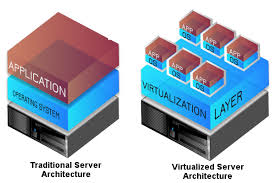
\includegraphics[height=4cm]{virtualization}
				\caption{Vista a confronto tra un ambiente server bare metal e virtualizzato. Immagine tratta da: http://bit.ly/2qvtLLk.}
			\end{center}
		\end{figure}
		
	 
 	\end{itemize} 
	\item \textbf{IT Governance}\\
	\begin{itemize}
		\item \textbf{Service management}\\
		Un servizio informatico richiede costante attenzione. Questo necessita di enormi investimenti 
		economici per la manutenzione. IKS offre diversi piani di gestione per soddisfare anche i più 
		esigenti clienti;
	    
	    \begin{figure}[htbp]
	    	\begin{center}
	    		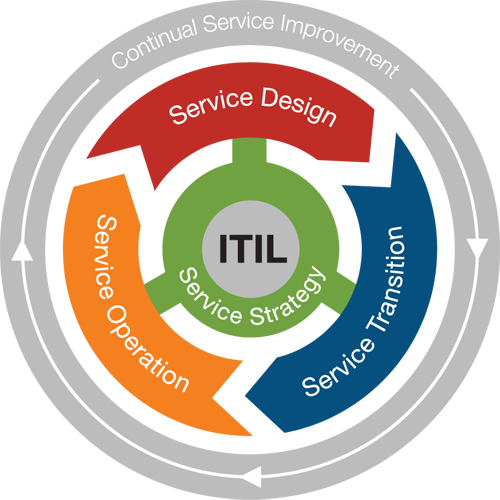
\includegraphics[height=5cm]{itil}
	    		\caption{Visione della gestione di servizio in prospettiva del \gls{framework} ITIL. Immagine tratta da: http://bit.ly/2qvNryk.}
	    	\end{center}
	    \end{figure}
	    
	    \newpage  
		\item \textbf{Application and performance monitoring}\\ 
		Un prodotto software ha il proprio specifico ciclo di vita. Concluso il ciclo di sviluppo, 
		il prodotto è rilasciato in produzione. La seconda parte del ciclo di vita di un prodotto 
		software è la manutenzione. Essere in grado di monitorare un applicativo è importante per 
		avere una costante visione dello stato del prodotto e prevenire eventuali esigenze di 
		manutenzione generica oppure di basso profilo a livello di codice sorgente. In questo 
		dominio, grazie a partnership strategiche, IKS offre soluzioni mirate a garantire la miglior 
	    possibile esperienza di monitoraggio applicativo;
	
	
		\item \textbf{System and networking management}\\
		Gestire sistemi e reti complessi è un compito complesso. Utilizzare strumenti adeguati 
		permette di semplificare il lavoro e garantire un stato consistente del sistema nel tempo. Le 
		soluzioni offerte di IKS sono orientate alla flessibilità e facilità d'uso dei prodotti 
		offerti in questo contesto;
	\end{itemize} 
	\item \textbf{Innovation \& Project} \\
	\begin{itemize}
		\item \textbf{Architetture applicative distribuite}\\
		I sistemi informatici diventano sempre più di natura distribuita. IKS offre in questo 
		ambito soluzioni architetturali orientate a microservizi, utilizzando le ultime 
		tecnologie orientate alla containerizzazione e orchestrazione di container; 
	
	
		\item \textbf{Sviluppo di applicazioni cloud native}\\
		E' sempre più comune sentire parlare di cloud. Le classiche architetture applicative 
		non riescono a beneficiare della flessibilità del cloud perché non sono scalabili e sono 
		difficilmente modularizzabili vista la loro architettura a monolite. Per questo motivo
		le applicazioni devono essere sviluppate fin dal principio con un'architettura orientata 
		al Cloud. Una buona guida di sviluppo di applicazioni web orientate al Cloud è la 
		\textit{Twelve Factor-Factor App}. In questa direzione IKS si impegna di proporre 
		soluzioni architetturali orientate all'affidabilità, resilienza, scalabilità orizzontale ed ecc.
		
		\begin{figure}[htbp]
			\begin{center}
				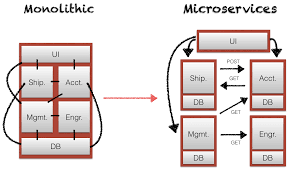
\includegraphics[height=5cm]{monolith-microservice}
				\caption{Visione architetturale a monolite e microservizi a confronto. Immagine tratta da: http://bit.ly/2rh1niY.}
			\end{center}
		\end{figure}
	\end{itemize} 
\end{itemize}

La clientela tipica di IKS sono aziende che operano nell'ambito 
della pubblica amministrazione, bancario, assicurativo e servizi. 

Una lista dettagliata delle referenze può essere consultata sul sito
di IKS all'URL \url{https://www.iks.it/referenze.html}.


\subsection{Struttura organizzativa}

Ad oggi IKS conta più di 100 dipendenti. La sua organizzazione interna è 
riassunta nel diagramma in \textbf{Figura 1.8}.

In seguito descrivo le unità operative che costituiscono il nucleo decisionale dell'azienda. 
Queste unità sono:
\begin{itemize}
	\item \textbf{Direzione}\\ 
	Definisce gli orientamenti e le politiche aziendali. Definisce gli obiettivi 
	per la qualità, riesamina periodicamente il sistema di qualità e gestisce 
	il piano di formazione dei dipendenti in funzione alle esigenze e motivazioni 
	personali;
	\item \textbf{Direzione Commerciale}\\
	Definisce le politiche commerciali, gli obiettivi e le risorse necessarie.
	Promuove i servizi e prodotti dell'azienda. Gestisce i clienti, i fornitori 
	e le offerte contrattuali;
	\item \textbf{Direzione tecnica o Operation}\\
	Supporta la Direzione Commerciale nella valutazione commerciale di prodotti 
	e/o offerte dal punti di vista tecnico. Gestisce a livello tecnico i progetti 
	e servizi. Pianifica le risorse necessarie per i prodotti/servizi. Verifica 
	lo stato del prodotto/servizio offerto;	
	\item \textbf{Amministrazione \& Finanza}\\
	Gestisce la documentazione di progetto su coordinamento della direzione 
	commerciale e tecnica. Gestisce l'archiviazione della documentazione;
	\item \textbf{Acquisti}\\
	Su coordinamento della Direzione, gestisce i fornitori di prodotti e servizi. 
	Gestisce il processo di acquisizione di nuovi prodotti o servizi. Il 
	processo di acquisizione è guidato dalle necessità interne aziendali oppure 
	da quelle dei clienti;
	\item \textbf{Assicurazione Qualità}\\
	E' i stretto contatto solo con la Direzione. Gestisce il piano di qualità, 
	coordina le attività di ispezione, misura e stima il livello della 
	qualità aziendale;
	\item \textbf{Business Unit (BU)}\\
	Gestisce i progetti o servizi concordati con il Cliente. Rendiconta 
	direttamente alla Direzione Tecnica e gestisce l'emissione delle 
	fatture verso il Cliente. 
\end{itemize}


\begin{figure}[htbp]
	\begin{center}
		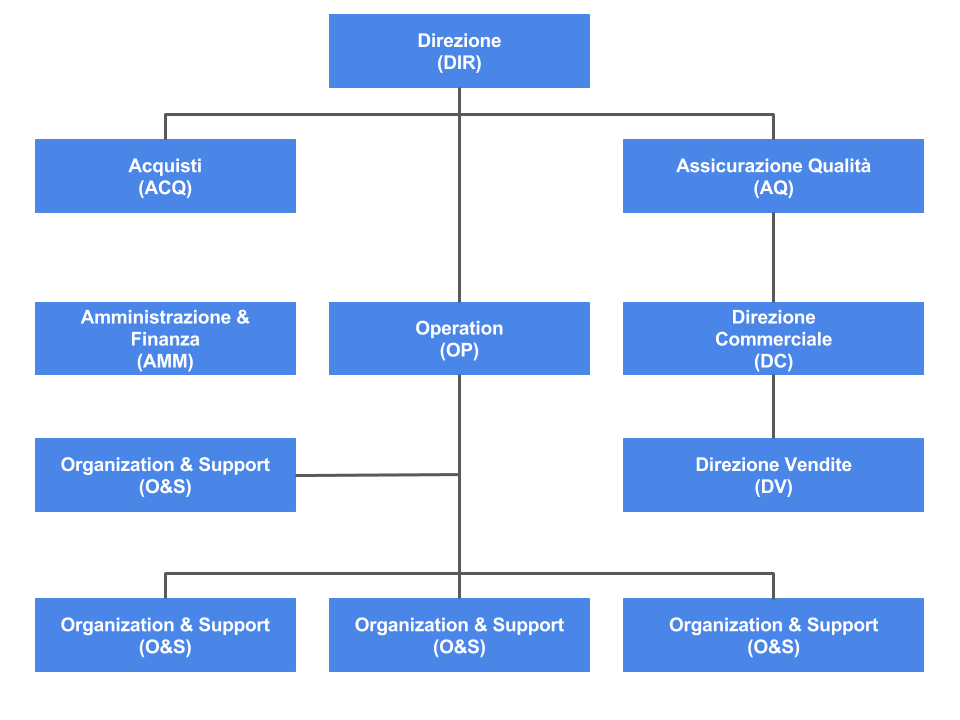
\includegraphics[height=8cm]{organigramma}
		\caption{Organigramma aziendale}
	\end{center}
\end{figure}



\subsection{Processi aziendali}

IKS dal 2003 è certificata UNI EN ISO 9001. Questo certifica che 
l'azienda cura molto la qualità del lavoro interno. Infatti, migliorare di continuo 
il proprio \textit{modus operandis} permette all'azienda di rimanere competitiva sul mercato 
e consolidare la propria posizione di leader sul mercato del ICT italiano. 
Riporto di seguito alcuni obiettivi di qualità dell'azienda:
\begin{itemize}
	\item Mantenere e aumentare il livello di soddisfazione del Cliente;
	\item Operare in modo efficiente ed efficace per soddisfare i requisiti contrattuali, 
	      norme e regolamenti;
	\item Monitorare i propri processi per garantire azioni correttive 
	      tempestivamente e permettere un comportamento pro attivo, per 
	      anticipare i bisogni e predire le risorse aziendali necessarie 
	      prima del loro effettivo bisogno; 
	\item Assicurare una adeguata formazione al Personale.
\end{itemize}


Il ruolo del Cliente è di prima importanza. Infatti, l'azienda cerca di coinvolgerlo
il più possibile per comprendere meglio i suoi bisogni. Dopo aver formalizzato 
il bisogno del Cliente segue un'attività di analisi dei requisiti. L'obiettivo dell'attività 
è la dettagliata comprensione del contesto applicativo, quali sono le parti interagenti e quali 
possono essere i rischi durante l'attività di progetto per implementare i bisogni del Cliente.

A progetto concluso, il Cliente valuta criticamente la soluzione presentata. 
La valutazione può coinvolgere anche un reclamo, il quale è rivolto alla Direzione dell'azienda.

IKS organizza il proprio lavoro per processi: primari, direttivi e di supporto. Ciascuna categoria 
di processo definisce delle responsabilità e compiti. Per esempio i processi organizzativi interessano 
le attività per: definire la politica e strategia aziendale, pianificare e allocare le risorse, 
riesaminare la gestione del sistema di qualità. Invece, i processi primari ricoprono attività 
che garantiscono un diretto ricavo economico per l'azienda e danno un valore aggiunto al prodotto
o servizio fornito. Esempi di attività sotto questa categoria sono: proporre offerte commerciali ai 
clienti, progettare e sviluppare  prodotti software, erogare servizi IT.
L'ultima categoria di processi sono quelli di supporto. Tra le consone attività giornaliere rientrano
le seguenti, per esempio: gestire le risorse umane, l'infrastruttura e gli ambienti di lavoro, 
monitorare e analizzare la qualità aziendale. 

Una rappresentazione grafica di come sono legate le parte durante un progetto segue in \textbf{Figura 1.9}.

Periodicamente il responsabile della qualità su mandato della Direzione attua attività 
d'ispezione per controllare la qualità. A posteriori segue un'attività di analisi e 
misura i livelli di qualità per ogni reparto interno, servizio e prodotto di IKS.

\begin{figure}[htbp]
	\begin{center}
		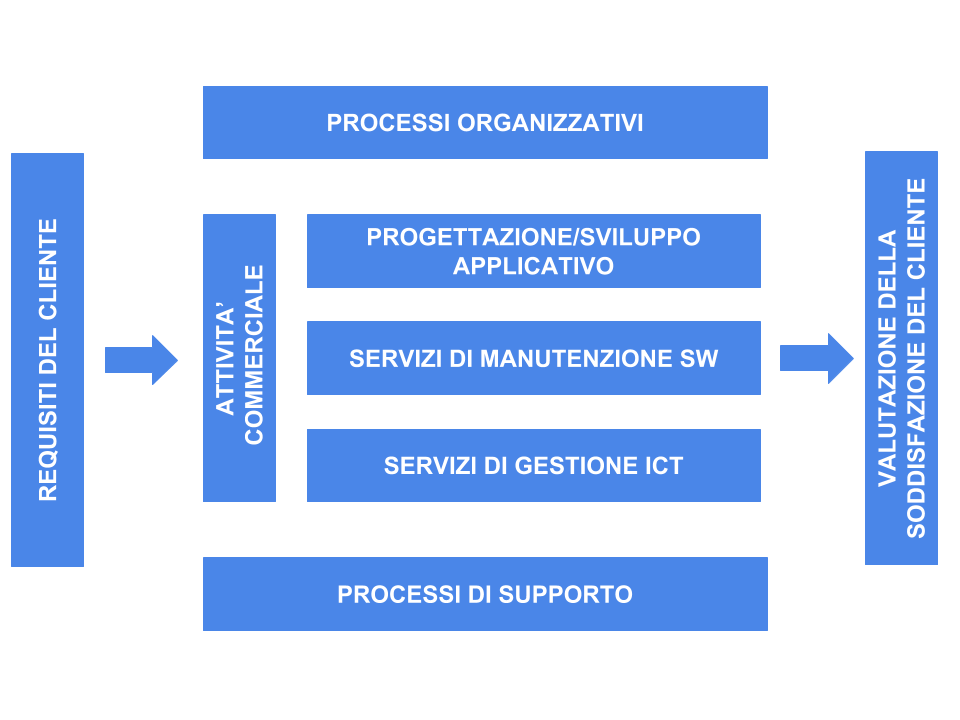
\includegraphics[height=7cm]{relazione-responsabilita}
		\caption{Rappresentazione grafica del coinvolgimento del Cliente e i corrispettivi livelli degli interventi 
			del gruppo commerciale, tecnico, direzionale e di supporto nella gestione di un'offerta di progetto.}
	\end{center}
\end{figure}



% Parte tre del capitolo
\section{Rapporto con l'innovazione}
L'innovazione è il processo di gestione dell'intero ciclo di vita di un'idea. 
L'obiettivo è portare un miglioramento di processo aziendale, di prodotto e/o 
di servizio. Il seguente miglioramento si traduce in un valore aggiunto per l'azienda 
in termini di rientro economico e per il Cliente nel soddisfare un bisogno in modo più
efficace ed efficiente. 

L'approccio innovativo induce l'utilizzo dell'informazione, della creatività e dello spirito 
d'iniziativa per raccogliere maggior valore aggiunto dalle risorse a disposizione. L'azienda 
utilizza l'innovazione per soddisfare in modo pro attivo le richieste del Cliente. Questo principio
è pienamente il linea con la strategia di qualità aziendale: \textit{client first}.

La modalità di innovazione di IKS è un approccio incrementale. Inizialmente l'azienda cerca di 
soddisfare i bisogni principali e raggiungere il prima possibile gli obiettivi fissati. In seguito, 
l'azienda si impegna di migliorare la propria offerta mediante miglioramenti continui a ogni 
livello di dettaglio. 

Per supportare l'innovazione IKS ha creato una cultura aziendale che permette ai propri dipendenti
di scambiarsi idee, sperimentare, imparare in gruppo e mettere in atto la propria creatività.
Non manca la comunicazione con i propri responsabili. Questi sono i primi a motivare di continuo 
le risorse umane a loro disposizione. Il dialogo dipendente-responsabile non è verticale. La cultura 
aziendale in questa direzione è molto drastica: favorire uno scambio di idee equo, semplice e rompere 
le gerarchie. 

In questo contesto, per l'intera durata del mio periodo di stage e dopo un primo momento di 
ambientamento ho beneficiato molto del clima aziendale. Infatti, non è mancato il libero 
confronto con il tutor aziendale che si è mostrato molto disponibile e aperto al mio spirito
d'iniziativa. Lui mi ha supportato in ogni scelta che io ho motivato e ritenuto significativo 
per il beneficio del mio progetto. 

Le idee sono una parte del processo di gestione dell'innovazione: la realtà è molto più 
complessa. IKS non possiede un effettivo processo di gestione a livello aziendale. Questo 
viene gestito da un gruppo di persone con competenze trasversali e a livelli organizzativi 
differenti. 

\begin{figure}[htbp]
   \begin{center}
	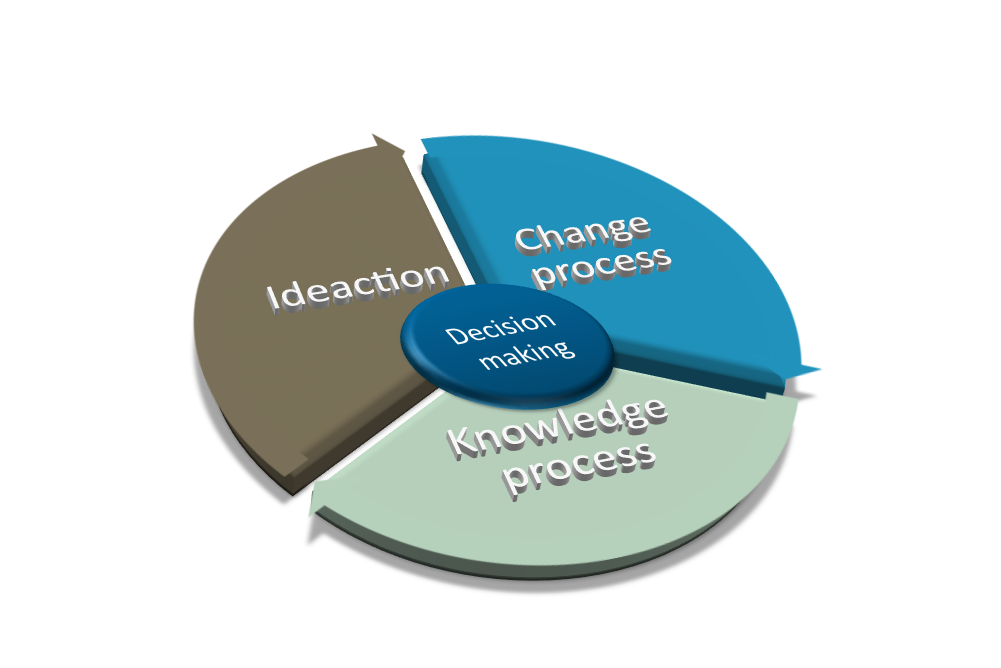
\includegraphics[height=5cm]{innovation-management}
	\caption{Il legame attivo tra innovazione e il processo del cambiamento e gestione della conoscenza. Immagine tratta da: http://bit.ly/2qty3XD.}
   \end{center}
\end{figure}


\newpage 


%\begin{description}
%	\item[{\hyperref[cap:processi-metodologie]{Il secondo capitolo}}] descrive ...
%	
%	\item[{\hyperref[cap:descrizione-stage]{Il terzo capitolo}}] approfondisce ...
%	
%	\item[{\hyperref[cap:analisi-requisiti]{Il quarto capitolo}}] approfondisce ...
%	
%	\item[{\hyperref[cap:progettazione-codifica]{Il quinto capitolo}}] approfondisce ...
%	
%	\item[{\hyperref[cap:verifica-validazione]{Il sesto capitolo}}] approfondisce ...
%	
%	\item[{\hyperref[cap:conclusioni]{Nel settimo capitolo}}] descrive ...
%\end{description}


%Riguardo la stesura del testo, relativamente al documento sono state adottate le seguenti convenzioni tipografiche:
%\begin{itemize}
%	\item gli acronimi, le abbreviazioni e i termini ambigui o di uso non comune menzionati vengono definiti nel glossario, situato alla fine del presente documento;
%	\item per la prima occorrenza dei termini riportati nel glossario viene utilizzata la seguente nomenclatura: \emph{parola}\glsfirstoccur;
%	\item i termini in lingua straniera o facenti parti del gergo tecnico sono evidenziati con il carattere \emph{corsivo}.
%\end{itemize}

